%%%%%%%%%%%%%%%%%%%%%%%%%%%%%
%Update: <Sep/24/2010>
%%%%%%%%%%%%%%%%%%%%%%%%%%%%%
\chapter{マイクロコンピュータ応用}

\section{目的}

拡張パラレルIOボードの使い方を学び, 拡張パラレルIOボードにステッピングモータをつ
なぎ制御する。さらにスイッチも同時に制御することを目標とする。

\section{装置}
\subsection{拡張パラレルIOボード}

マイコントレーナには1つのIOポートが付いています。しかし,
2つ以上の拡張ボードを接続する必要が生じることがあります。
MT-Zでは本演習で用いるパラレルIOボードを接続することで, 2つのIOポートを増やすことができます。

\subsection{装置セッティング}

まず\figref{fig:connection-io}のように, MT-Zの左下にあるバスコネクタに拡張パラレルIOボードを繋ぎます。
そして, ステッピングモータとアダプタをあらかじめ接続したステッピングモータインター
フェースボードをCH1に繋ぎます。

拡張パラレルIOボードは, 前学期用いた8255Aが2つ使われています。よって, 拡張パラレルIOボー
ドに接続した機器を使う場合, 前学期に習ったスイッチ, LEDなどの制御方法と同じよう
にコントロールワードを指定し, ポートに信号を送ってやれば動作します。
IOボードを使う場合の各ポートのアドレスは\tabref{tab:ch1}, \tabref{tab:ch2}のよう
になっています。ここでは, CH1の8255Aを用いるのでCH1のアドレスを用います。
プログラムを組むときには\tabref{tab:ch1}のアドレスを用いてください。
今回もコントロールワードは90Hを用います。

\begin{table}
\begin{minipage}{0.5\hsize}
\begin{center}
\caption{拡張パラレルIOボードCH1のポートアドレス}
\label{tab:ch1}
\begin{tabular}{|c|c|}
\hline
PA& 20H\\ \hline
PB& 21H\\ \hline
PC& 22H\\ \hline
CTRL& 23H\\
\hline
\end{tabular}
\end{center}
\end{minipage}
\begin{minipage}{0.5\hsize}
\begin{center}
\caption{拡張パラレルIOボードCH2のポートアドレス}
\label{tab:ch2}
\begin{tabular}{|c|c|}
\hline
PA& 24H\\ \hline
PB& 25H\\ \hline
PC& 26H\\ \hline
CTRL& 27H\\
\hline
\end{tabular}
\end{center}
\end{minipage}
\end{table}

\begin{figure}[htbp]
\begin{center}
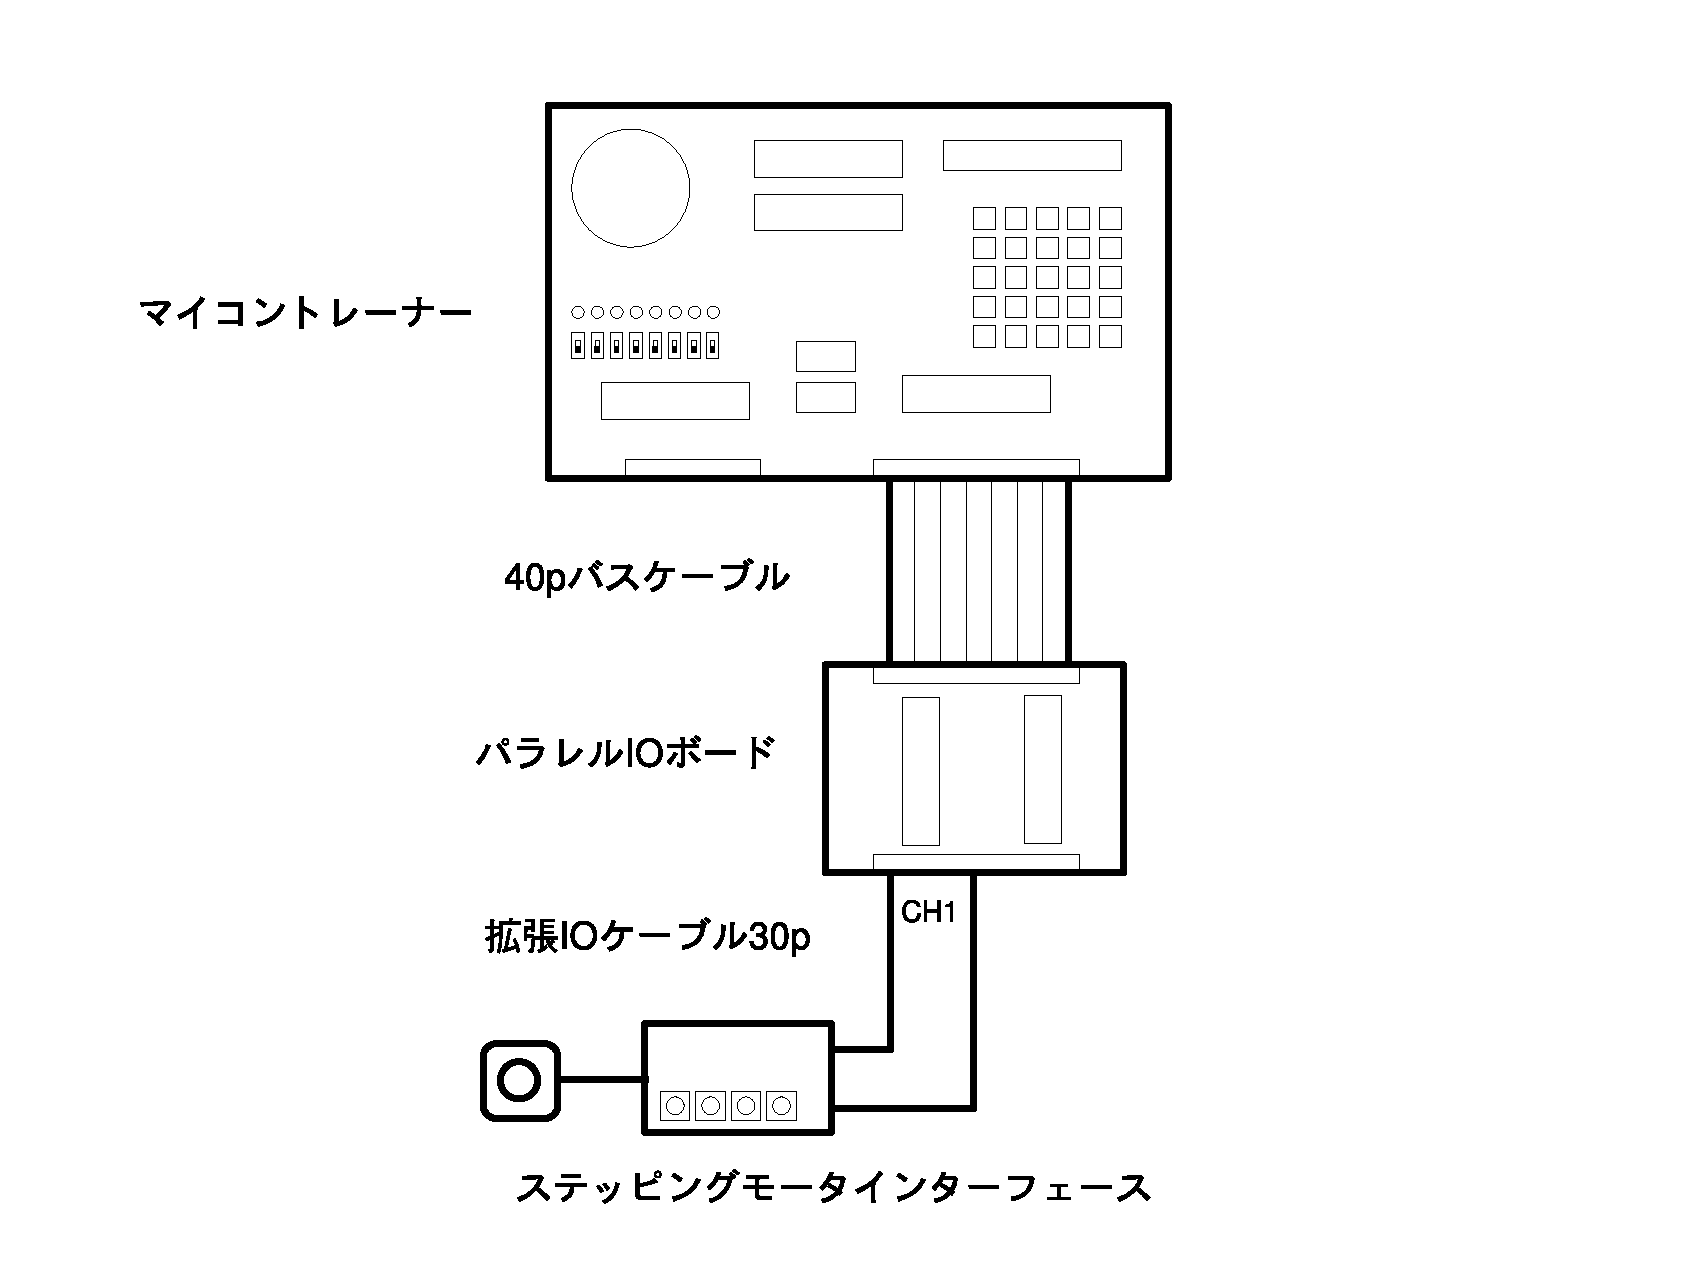
\includegraphics[width=1\linewidth]{img/connection-io.eps}
\caption{装置の接続の様子。}
\label{fig:connection-io}
\end{center}
\end{figure}

\newpage

\section{実験}

\begin{description}
\item[課題1] 拡張パラレルIOボードに接続したステッピングモータを1相励磁回転で回転させなさい(\tabref{tab:q3-1})。
           プログラムは, 前回のステッピングモータ制御プログラムの, 出力ポートアドレスを\tabref{tab:ch1}を参考
           に修正することでステッピングモータは動きます。

\begin{table}
\begin{center}
\caption{課題1のプログラム}
\label{tab:q3-1}
\footnotesize
\begin{tabular}{|c|l|ll|l|}
\hline
アドレス& \multicolumn{1}{|c|}{機械語}&\multicolumn{1}{|c}{ラベル}&\multicolumn{1}{c|}{ニーモニック}&\multicolumn{1}{|c|}{コメント}\\
\hline
   0005 &            &   &PB EQU 21H& 拡張IOポートBアドレス\\
   0007 &            &   &CTL EQU 23H& 拡張IOコントロールポートアドレス\\
   0090 &            &   &CLWD EQU 90H& 拡張IOコントロールワード\\
        &            &   &&\\
   8400 &            &   &    ORG 8400H&\\
   8400 &  \underline{~~~~} \underline{~~~~}     &   STPMTR:& LD A , CLWD& コン
                    トロールワードをAレジスタに転送\\
   8402 &  \underline{~~~~} \underline{~~~~}      &   &    OUT (CTL) , A & Aレジ
                    スタの値をコントロールポートに出力\\
   8404 &  \underline{~~~~} \underline{~~~~}       &   LOOP:& LD A , 01H& 01HをA
                    レジスタに転送\\
   8406 &  \underline{~~~~} \underline{~~~~}      &   &   OUT (PB) , A   & Aレジ
                    スタの値をポートBに出力\\
   8408 &  \underline{~~~~} \underline{~~~~}  \underline{~~~~}   &   &   CALL
                TIMER&  タイマを呼び出す\\
   840B &  \underline{~~~~} \underline{~~~~}      &   &   LD A , 02H& 02HをAレジ
                    スタに転送\\
   840D &  \underline{~~~~} \underline{~~~~}     &   &   OUT (PB) , A  & Aレジス
                タの値をポートBに出力\\
   840F &  \underline{~~~~} \underline{~~~~} \underline{~~~~}  &   &   CALL
                TIMER&タイマを呼び出す\\
   8412 &  \underline{~~~~} \underline{~~~~}     &   &   LD A , 04H& 04HをAレジ
                    スタに転送\\
   8414 &  \underline{~~~~} \underline{~~~~}      &   &   OUT (PB) , A   & Aレジ
                    スタの値をポートBに出力\\
   8416 &  \underline{~~~~} \underline{~~~~} \underline{~~~~}   &   &   CALL
                TIMER& タイマを呼び出す\\
   8419 &  \underline{~~~~} \underline{~~~~}      &   &   LD A , 08H& 08HをAレジ
                    スタに転送\\
   841B &  \underline{~~~~} \underline{~~~~}     &   &   OUT (PB) , A& Aレジスタ
                    の値をポートBに出力\\
   841D &  \underline{~~~~} \underline{~~~~} \underline{~~~~}   &   &   CALL
                TIMER& タイマを呼び出す\\
   8420 &  \underline{~~~~} \underline{~~~~} \underline{~~~~}   &   &   JP LOOP& ループにジャン
                    プ\\
        &            &   &&\\
   8440 &            &    &    ORG 8440H&\\
   8440 &  21 00 40   &    TIMER:& LD
                HL , 4000H& 値4000HをHLレジスタに転送\\
   8443 &  5F        &    &    LD E, A&Aレジスタの値をEレジスタに
                    転送\\
   8444 &  2B        &    TLOOP:& DEC HL&HLレジスタの値から1を引く\\
   8445 &  7C        &    &    LD A, H&Hレジスタの値をAレジスタに
                    転送\\
   8446 &  B5        &    &    OR L& Aの値とLの値の論理和をとる\\
   8447 &  20 FB       &    &    JR NZ , TLOOP& フ
                    ラグレジスタがNZならばTLOOPにジャンプ\\
   8449 &  7B        &    &    LD A, E& Eレジスタの値をAレジスタに
                    転送\\
   844A &  C9        &    &    RET&ルーティンの終了\\
   844B &            &    &    END&\\

\hline
\end{tabular}
\end{center}
\end{table}


\item[課題2] 課題1で作ったプログラムを改造し, 速度をいろいろと変えてみなさい。

\item[課題3] 課題1で作ったプログラムを改造し, 逆回転させなさい。

\item[課題4] 右端のスイッチがONの場合高速回転, OFFの場合は低速回転するプログラム
           を作りなさい(\tabref{tab:q3-4-1}, \ref{tab:q3-4-2})。

\begin{table}
\begin{center}
\caption{課題4のプログラム}
\label{tab:q3-4-1}
\footnotesize
\begin{tabular}{|c|l|ll|l|}
\hline
アドレス& \multicolumn{1}{|c|}{機械語}&\multicolumn{1}{|c}{ラベル}&\multicolumn{1}{c|}{ニーモニック}&\multicolumn{1}{|c|}{コメント}\\
\hline
   0004 &          &  & PA EQU 04H& オンボード8255AポートAアドレス\\
   0005 &          &  & PB EQU 05H& オンボード8255AポートBアドレス\\
   0007 &          &  & CTL EQU 07H& オンボード8255Aコントロールポートアドレス\\
   0090 &          &  & CLWD EQU 90H& オンボード8255Aコントロールワード\\
   0021 &          &  & PB2 EQU 21H& 拡張IOポートBアドレス\\
   0023 &          &  & CTL2 EQU 23H& 拡張IOコントロールポートアドレス\\
   0090 &          &  & CTLW2 EQU 90H& 拡張IOコントロールワード\\
     &          &  & &\\
   8400 &          &  &     ORG 8400H&\\
   8400 & \underline{~~~~} \underline{~~~~}    &  &    LD A, CLWD& オンボード
                    8255A用コントロール
                    ワードをAレジスタに転送\\
   8402 & \underline{~~~~} \underline{~~~~}    &  &     OUT (CTL), A& Aレジスタ
                    の値をオンボード8255Aコントロールポートに出力\\
   8404 & \underline{~~~~} \underline{~~~~}     &  &     LD A , CTLW2& 拡張IOコ
                    ントロールワードをAレジスタに転送\\
   8406 & \underline{~~~~} \underline{~~~~}    &  &     OUT (CTL2) , A& Aレジス
                    タの値を拡張IOコントロールポートに出力\\
   8408 & \underline{~~~~} \underline{~~~~} \underline{~~~~}  &  &     LD DE,
                4000H& 4000HをDEレジスタに転送\\
   840B & \underline{~~~~} \underline{~~~~} \underline{~~~~} &   LOOP:& CALL
                MOTOR& モータを呼び出す\\
   840E & \underline{~~~~} \underline{~~~~}     &  &     IN A, (PA)& ポートAの状
                    態をAレジスタに入力\\
   8410 & \underline{~~~~} \underline{~~~~}    &  &     AND 01H& 01Hとの論理積を
                    とる\\
   8412 & \underline{~~~~} \underline{~~~~}     &  &     CP 00H& 00と比較する\\
   8414 & \underline{~~~~} \underline{~~~~} \underline{~~~~}  &  &     JP Z,
                SLOW& フラグレジスタがZならばSLOWにジャンプ\\
   8417 & \underline{~~~~} \underline{~~~~} \underline{~~~~} &  &     JP FAST&
                    FASTにジャンプ\\
        &          &  &     &\\
   841A & \underline{~~~~} \underline{~~~~}    &   MOTOR&    LD A , 01H& 01HをA
                    レジスタに転送\\
   841C & \underline{~~~~} \underline{~~~~}     &  &     OUT (PB2) , A& Aレジス
                    タの値を拡張IOポートBに出力\\
   841E & \underline{~~~~} \underline{~~~~} \underline{~~~~} &  &     CALL
                TIMER& タイマを呼び出す\\
   8421 & \underline{~~~~} \underline{~~~~}     &  &     LD A , 02H& 02HをAレジ
                    スタに転送\\
   8423 & \underline{~~~~} \underline{~~~~}    &  &     OUT (PB2) , A& Aレジスタ
                    の値を拡張IOポートBに出力\\
   8425 & \underline{~~~~} \underline{~~~~} \underline{~~~~} &  &     CALL
                TIMER& タイマを呼び出す\\
   8428 & \underline{~~~~} \underline{~~~~}    &  &     LD A , 04H& 04HをAレジス
                    タに転送\\
   842A & \underline{~~~~} \underline{~~~~}    &  &     OUT (PB2) , A & Aレジス
                    タの値を拡張IOポートBに出力\\
   842C & \underline{~~~~} \underline{~~~~} \underline{~~~~}  &  &     CALL
                TIMER&タイマを呼び出す\\
   842F & \underline{~~~~} \underline{~~~~}     &  &     LD A , 08H& 08HをAレジス
                    タに転送\\
   8431 & \underline{~~~~} \underline{~~~~}     &  &     OUT (PB2) , A & Aレジス
                    タの値を拡張IOポートBに出力\\
   8433 & \underline{~~~~} \underline{~~~~} \underline{~~~~}  &  &     CALL TIMER&タイマを呼び出す\\
   8436 & \underline{~~~~}       &  &     RET& ルーティン終了\\
        &          &  &     &\\
   8437 & \underline{~~~~} \underline{~~~~} \underline{~~~~}  &  SLOW:& LD DE, 1000H&\\
   843A & \underline{~~~~} \underline{~~~~} \underline{~~~~} &  &     JP LOOP&\\
        &          &  & &\\
   843D & \underline{~~~~} \underline{~~~~} \underline{~~~~} &  FAST:& LD DE, 300H&\\
   8440 & \underline{~~~~} \underline{~~~~} \underline{~~~~} &  &     JP LOOP&\\
        &          &  &     &\\

\hline
\end{tabular}
\end{center}
\end{table}


\begin{table}
\begin{center}
\caption{課題4のプログラムの続き}
\label{tab:q3-4-2}
\footnotesize
\begin{tabular}{|c|l|ll|l|}
\hline
アドレス& \multicolumn{1}{|c|}{機械語}&\multicolumn{1}{|c}{ラベル}&\multicolumn{1}{c|}{ニーモニック}&\multicolumn{1}{|c|}{コメント}\\
\hline
       &          &  &     &\\
   8600 &          &  &     ORG 8600H&\\
   8600 & \underline{~~~~}       &   TIMER:& LD H, D&\\
   8601 & \underline{~~~~}       &  &     LD L, E&\\
   8602 &  5F        &    &    LD E, A&Aレジスタの値をEレジスタに
                    転送\\
   8603 &  2B        &    TLOOP:& DEC HL&HLレジスタの値から1を引く\\
   8604 &  7C        &    &    LD A, H&Hレジスタの値をAレジスタに
                    転送\\
   8605 &  B5        &    &    OR L& Aの値とLの値の論理和をとる\\
   8606 &  20 FB       &    &    JR NZ , TLOOP& フ
                    ラグレジスタがNZならばTLOOPにジャンプ\\
   8608 &  7B        &    &    LD A, E& Eレジスタの値をAレジスタに
                    転送\\
   8609 &  C9        &    &    RET&ルーティンの終了\\
   860A &            &    &    END&\\


\hline
\end{tabular}
\end{center}
\end{table}

\item[課題5(発展)] 右端のスイッチをONにすると時計回りに回転し, OFFの時に反時計回りに
           回転させるプログラムを作りなさい。


\end{description}


\section{考察課題}
\begin{description}
\item[考察課題1] 回転速度を速くしたり, 遅くしたりしたときに, うまくモータが回転したか。おそ
      らく, うまく回転しなかった場合があると思われる。そのどのようなときにうまく
      回転しなかったか報告し, その原因が何か考えよ。
\item[考察課題2] 次回の課題プログラムの流れを考えよ。

\end{description}
